\chapter{Química del Agua}
El agua es un electrolito débil y es capaz de disociarse en una proporción muy escasa y originar tanto $H^{+}$, como $OH^{-}$.La disociación del $H_{2}O$, es la siguiente:
\begin{center}
	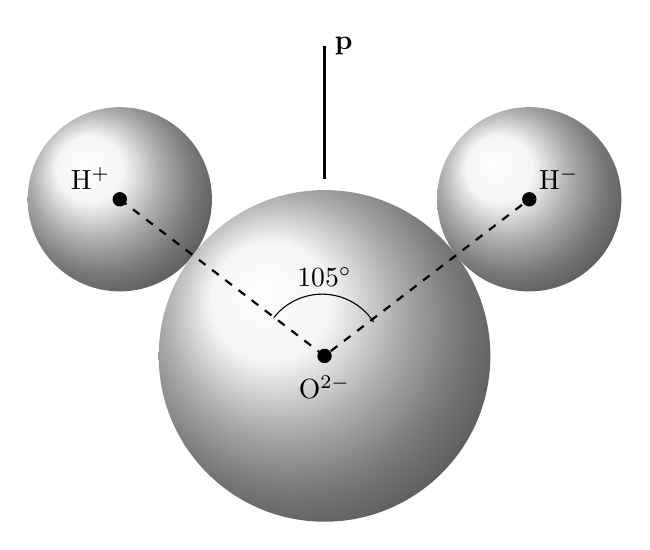
\begin{tikzpicture}[>=latex,scale=1.3]
		\shade[ball color=gray!10!] (0,0) coordinate(Hp) circle (.9) ;
		\shade[ball color=gray!10!] (2,-1.53) coordinate(O) circle (1.62) ;
		\shade[ball color=gray!10!] (4,0) coordinate(Hm) circle (.9) ;
		\draw[thick,dashed] (0,0) -- (2,-1.53) -- (4,0) ;
		\draw[thick] (2,.2) -- (2,1.5) node[right]{$\mathbf{p}$} ;
		\draw (2.48,-1.2) arc (33:142:.6)  ;
		\draw (2,-.95) node[above]{$105^{\circ}$} ;
		\draw (0,.2) node[left]{H$^+$} ;
		\draw (4,.2) node[right]{H$^-$} ;
		\draw (2,-1.63) node[below]{O$^{2-}$} ;
		\foreach \point in {O,Hp,Hm}
		  \fill [black] (\point) circle (2pt) ;
	  \end{tikzpicture}
\end{center}
\begin{equation}
	2H_{2}O \rightleftharpoons H_{3}O^{+} + OH^{-}
\end{equation}


\begin{gather*}
	K_{eq} = \frac{\left[ OH^{-} \right]  \left[ H^{+} \right]}{\left[H_{2}O\right] }\\
	K_{eq} \left[H_{2}O\right] = {\left[ OH^{-} \right]  \left[ H^{+} \right]} \\
	\left[ OH^{-} \right] = H^{+} = 10^{-7} \frac{M}{L}
\end{gather*}

\subsection{Formulación inorgánica}

\subsubsection{Grupos funcionales}

\begin{table}[h!]
	\centering
	\begin{tabular}{cccc}
		\hline
		Nombre      & Fórmula       & Nombre             & Fórmula   \\ \hline
		hidróxido   & $OH^{-}$      & $S^{2-}$           & sulfuro   \\
		cloruro     & $Cl^{-}$      & $CrO_{4}^{2-}$     & cromato   \\
		nitrato     & $NO_{3}^{-}$  & $PO_{4}^{3-}$      & fosfato   \\
		nitrito     & $NO_{2}^{-}$  & $Cr_{2}O_{7}^{2-}$ & dicromato \\
		bicarbonato & $HCO_{3}^{-}$ & $SO_{4}^{2-}$      & sulfato   \\
		carbonato   & $CO_{3}^{2-}$ &                    &           \\ \hline
	\end{tabular}
	\caption{Aniones monoatómicos y poliatómicos}
	\label{tabq1}
\end{table}

La tabla \ref{tabq1}, es fundamental pues nos sirven los oxianiones para saber la alcalinidad en agua,
la cual se mide con la concentración de carbonato, bicarbonato e hidróxido; Para la calidad del agua es con la concentración de cloruro,
también se determina cantidad de sulfato, los nutrientes en fertirriego es fosfato, nitrato y nitrito. Los indicadores de cloruro, cromato y
dicromato sirven para reacciones oxido-reducción.

\begin{table}
	\centering
	\begin{tabular}{cccccc}
		\hline
		Nombre                                                           & Fórmula           & Nombre                                                             & Fórmula           & Nombre                                                             & Fórmula              \\ \hline
		hidróxido                                                        & $OH^{-}$          & \begin{tabular}[c]{@{}c@{}}Cloruro \\ de magnesio\end{tabular}     & $MgCl_{2}$        & \begin{tabular}[c]{@{}c@{}} Carbonato \\ de amonio\end{tabular}    & $(NH_{4})_{2}CO_{3}$ \\
		\begin{tabular}[c]{@{}c@{}}Ácido \\ clorhídrico\end{tabular}     & $HCL$             & \begin{tabular}[c]{@{}c@{}}Nitrato \\ de magnesio\end{tabular}     & $Mg(NO_{3})_{2}$  & \begin{tabular}[c]{@{}c@{}} Sulfato \\ de amonio\end{tabular}      & $(NH_{4})_{2}SO_{4}$ \\
		\begin{tabular}[c]{@{}c@{}}Ácido\\  nítrico\end{tabular}         & $HNO_{3}$         & \begin{tabular}[c]{@{}c@{}}Bicarbonato \\ de magnesio\end{tabular} & $Mg(HCO_{3})_{2}$ & \begin{tabular}[c]{@{}c@{}} Cloruro \\ de mercurio\end{tabular}    & $HgCl_{2}$           \\
		\begin{tabular}[c]{@{}c@{}}Ácido \\ nitroso\end{tabular}         & $HNO_{2}$         & \begin{tabular}[c]{@{}c@{}}Carbonato \\ de magnesio\end{tabular}   & $MgCO_{3}$        & \begin{tabular}[c]{@{}c@{}} Ácido \\perclórico\end{tabular}        & $HClO_{4}$           \\
		\begin{tabular}[c]{@{}c@{}}Ácido \\ sulfúrico\end{tabular}       & $H_{2}SO_{4}$     & \begin{tabular}[c]{@{}c@{}}Oxido\\  de magnesio\end{tabular}       & $MgO$             & \begin{tabular}[c]{@{}c@{}} Trióxido \\de azufre\end{tabular}      & $SO_{3}$             \\
		\begin{tabular}[c]{@{}c@{}}Ácido \\ sulfuroso\end{tabular}       & $H_{2}SO_{3}$     & \begin{tabular}[c]{@{}c@{}}Hidróxido \\ de sodio\end{tabular}      & $NaOH$            & \begin{tabular}[c]{@{}c@{}}Monóxido \\ de carbono\end{tabular}     & $CO$                 \\
		\begin{tabular}[c]{@{}c@{}}Ácido \\ bórico\end{tabular}          & $H_{3}BO_{3}$     & \begin{tabular}[c]{@{}c@{}}Cloruro \\ de sodio\end{tabular}        & $NaCl$            & \begin{tabular}[c]{@{}c@{}}Dióxido \\ de carbono\end{tabular}      & $CO_{2}$             \\
		\begin{tabular}[c]{@{}c@{}}Ácido \\ ortofosfórico\end{tabular}   & $H_{3}PO_{4}$     & \begin{tabular}[c]{@{}c@{}}Nitrato \\ de sodio\end{tabular}        & $NaNO_{3}$        & \begin{tabular}[c]{@{}c@{}}Ácido \\ acético\end{tabular}           & $CH_{3}COOH$         \\
		\begin{tabular}[c]{@{}c@{}}Ácido \\ pirofosfórico\end{tabular}   & $H_{4}P_{2}O_{7}$ & \begin{tabular}[c]{@{}c@{}}Carbonato\\ de sodio\end{tabular}       & $Na_{2}CO_{3}$    & \begin{tabular}[c]{@{}c@{}}Cianuro \\ de hidrógeno\end{tabular}    & $HCN$                \\
		\begin{tabular}[c]{@{}c@{}}Ácido \\ metafosfórico\end{tabular}   & $HPO_{3}$         & \begin{tabular}[c]{@{}c@{}}Sulfato \\ de sodio\end{tabular}        & $Na_{2}SO_{4}$    & \begin{tabular}[c]{@{}c@{}}Permanganato \\ de potasio\end{tabular} & $KMnO_{4}$           \\
		\begin{tabular}[c]{@{}c@{}}Hidróxido \\ de calcio\end{tabular}   & $Ca(OH)_{2}$      & \begin{tabular}[c]{@{}c@{}}Cloruro \\ de potasio\end{tabular}      & $KCl$             & \begin{tabular}[c]{@{}c@{}}Fosfato \\ de amonio\end{tabular}       & $(NH_{4})_{3}PO_{4}$ \\
		\begin{tabular}[c]{@{}c@{}}Cloruro \\ de calcio\end{tabular}     & $CaCl_{2}$        & \begin{tabular}[c]{@{}c@{}}Hidróxido \\ de potasio\end{tabular}    & $KOH$             & \begin{tabular}[c]{@{}c@{}}Óxido \\ férrico\end{tabular}           & $Fe_{2}O_{3}$        \\
		\begin{tabular}[c]{@{}c@{}}Nitrato \\ de calcio\end{tabular}     & $Ca(NO_{3})_{2}$  & \begin{tabular}[c]{@{}c@{}}Carbonato \\ de potasio\end{tabular}    & $K_{2}CO_{3}$     & \begin{tabular}[c]{@{}c@{}}Óxido\\  ferroso\end{tabular}           & $FeO$                \\
		\begin{tabular}[c]{@{}c@{}}Bicarbonato \\ de calcio\end{tabular} & $NaHCO_{3}$       & \begin{tabular}[c]{@{}c@{}}Bicarbonato \\ de potasio\end{tabular}  & $KHCO_{3}$        & \begin{tabular}[c]{@{}c@{}}hidróxido \\ de aluminio\end{tabular}   & $Al(OH)_{3}$         \\
		\begin{tabular}[c]{@{}c@{}}Sulfato \\ de calcio\end{tabular}     & $CaSO_{4}$        & \begin{tabular}[c]{@{}c@{}}Nitrato \\ de potasio\end{tabular}      & $KNO_{3}$         & \begin{tabular}[c]{@{}c@{}}Dióxido \\ de silicio\end{tabular}      & $SiO_{2}$            \\
		\begin{tabular}[c]{@{}c@{}}Carbonato\\ de calcio\end{tabular}    & $CaCO_{3}$        & \begin{tabular}[c]{@{}c@{}}Fosfato \\ de potasio\end{tabular}      & $K_{2}HPO_{4}$    & \begin{tabular}[c]{@{}c@{}}Dióxido \\ de azufre\end{tabular}       & $SO_{2}$             \\
		\begin{tabular}[c]{@{}c@{}}Oxido \\ de calcio\end{tabular}       & $CaO$             & \begin{tabular}[c]{@{}c@{}}Hidróxido \\ de amonio\end{tabular}     & $NH_{4}OH$        & \begin{tabular}[c]{@{}c@{}}Sulfuro \\ de hidrógeno\end{tabular}    & $H_{2}S$             \\
		\begin{tabular}[c]{@{}c@{}}Hidróxido \\ de magnesio\end{tabular} & $Mg(OH)_{2}$      & \begin{tabular}[c]{@{}c@{}}Cloruro \\ de amonio\end{tabular}       & $NH_{4}Cl$        & \begin{tabular}[c]{@{}c@{}}Dicromato \\ de potasio\end{tabular}    & $K_{2}Cr_{2}O_{7}$   \\
		\begin{tabular}[c]{@{}c@{}}Nitrato\\ de amonio\end{tabular}      & $NH_{4}NO_{3}$    &                                                                    &                   &                                                                    &                      \\ \hline
	\end{tabular}
	\caption{Sales y ácidos}
	\label{tabq2}
\end{table}

\subsubsection{Disociaciones}
En la tabla \ref{tabq2}, contiene sales y ácidos que son  de suma importancia en la química de agua, pues nos sirven como indicadores.


\section{Conceptos fundamentales de la química del agua}
Se usaron definiciones dadas del libro Química\autocite{chang2013}, escrito por Raymond Chang \& Kenneth A. Goldsby:
\begin{definition}[Átomo]
	Es la unidad básica de un
	elemento que puede intervenir en una combinación química.
\end{definition}

\begin{definition}[Molécula]
	Una molécula es un agregado de, por lo menos, dos átomos en una colocación definida
	que se mantienen unidos a través de fuerzas químicas (también llamadas enlaces químicos).
\end{definition}

\begin{definition}[Ión]
	Un ion es un átomo o un grupo de átomos que tiene una carga neta positiva o negativa.
	El número de protones, cargados positivamente, del núcleo de un átomo permanece igual
	durante los cambios químicos comunes (llamados reacciones químicas), pero se pueden
	perder o ganar electrones, cargados negativamente.
\end{definition}

\begin{definition}[Número de oxidación ]
	significa el número de cargas que tendría
	un átomo en una molécula (o en un compuesto iónico)
	si los electrones fueran transferidos completamente.
\end{definition}

\begin{definition}[Peso atómico]
	se define como una masa exactamente igual a un doceavo de la masa de un
	átomo de carbono-12. El carbono-12 es el isótopo del carbono que tiene seis protones y
	seis neutrones. Al fijar la masa del carbono-12 como 12 uma, se tiene el átomo que se
	utiliza como referencia para medir la masa atómica de los demás elementos.
\end{definition}

\begin{definition}[Masa molar]
	es una propiedad física definida como su masa por unidad de cantidad de sustancia.
\end{definition}

\begin{definition}[Equivalentes por mol]
	En las reacciones de precipitación, los equivalentes por mol dependerán de la
	carga eléctrica del ion implicado.
\end{definition}

\begin{definition}[Peso equivalente]
	Los pesos equivalentes $(P_{e})$ fueron determinados
	originalmente de forma experimental, pero
	(tal como se utilizan ahora) se obtienen de la
	división entre las masas molares $(mm=\frac{g}{mol})$
	y el número de oxidación del compuesto $(n)$.
	\begin{equation}
		P_{e}=\frac{mm}{n}
	\end{equation}
\end{definition}

\begin{definition}[Elemento químico]
	es una sustancia que no se puede separar en otras más sencillas por
	medios químicos. Hasta la fecha se han identificado 118 elementos. La mayoría de éstos se encuentran de manera natural en la Tierra.
	Los otros se han obtenido por medios científicos mediante procesos nucleares
\end{definition}

\begin{definition}[Compuesto químico]
	Los compuestos contienen átomos de diferentes
	elementos combinados en proporción de números enteros,
	y que los átomos no se crean ni se destruyen durante las
	reacciones químicas (ley de la conservación de la masa).
\end{definition}

\begin{definition}[Gas]
	Es una sustancia que habitualmente se encuentra en estado gaseoso
	a temperaturas y presiones normales; un vapor es la forma gaseosa
	de cualquier sustancia que sea un líquido o sólido a temperatura y presión normales.
\end{definition}

\begin{definition}[Líquido]
	Es una sustancia líquida, tiene sus moléculas cerca unas de otras,
	sin que se mantengan en una posición rígida, por lo que
	pueden moverse.
\end{definition}

\begin{definition}[Sólido]
	En un sólido, las moléculas ocupan una posición rígida y prácticamente no tienen
	libertad para moverse. Muchos sólidos tienen como característica un ordenamiento de
	largo alcance , es decir, sus moléculas están distribuidas en una configuración regular tridimensional
\end{definition}


\begin{definition}[Oxidación]
	El término reacción de oxidación se refiere a la semirreacción que implica la pérdida de electrones. En la antigüedad, los químicos empleaban el término “oxidación” para
	expresar la combinación de elementos con oxígeno. Sin embargo, actualmente tiene un
	significado más amplio, ya que también incluye reacciones en las que no participa el
	oxígeno
\end{definition}

\begin{definition}[Agente oxidante]
	Los agentes oxidantes siempre se reducen porque acepta electrones de otro átomo y
	hace que este se oxide.
\end{definition}

\begin{definition}[Reducción]
	Una reacción de reducción es una semirreacción que implica una ganancia de electrones.
\end{definition}

\begin{definition}[Agente reductor]
	Se dice que actúa como agente reductor porque dona electrones al oxígeno, siempre se oxidan.
	y hace que se reduzca
\end{definition}


\begin{definition}[Punto de ebullición]
	Es una propiedad física que indica un límite de temperatura para que un compuesto cambie de un estado
	líquido o sólido a gaseoso.
\end{definition}

\begin{definition}[Punto de fusión]
	Es una propiedad física que indica un límite de temperatura para que un compuesto cambie de
	estado sólido a líquido.
\end{definition}

\begin{definition}[Solución]
	Una disolución es una mezcla homogénea de dos o más sustancias. El soluto es la sustancia presente en menor cantidad, y el disolvente es la sustancia que está en mayor
	cantidad.
\end{definition}

\begin{definition}[Disolución]
	Es una mezcla homogénea de composición constante, se compone de soluto y disolvente.
\end{definition}

\begin{definition}[Solución saturada]
	Son aquellas en las que no se puede seguir admitiendo
	más soluto, pues el solvente ya no lo puede disolver.
	Si la temperatura aumenta, la capacidad para admitir
	más soluto aumenta.
\end{definition}

\begin{definition}[Electrolito débil]
	Una disolución de un electrólito débil contiene un pequeño número de iones
\end{definition}


\begin{definition}[Ácido]
	El ácido es un electrolito, una sustancia que libera iones hidrógeno $(H^{+})$
	se pueden ionizar completamente en agua.
\end{definition}


\begin{definition}[Base sal]
	Una base se describe como una sustancia que libera iones hidróxido $(OH^{-})$
	cuando está disuelta en agua.
\end{definition}

\begin{definition}[Neutralización]
	es una reacción entre un ácido y una base. Generalmente, en las reacciones acuosas ácido-base se forma agua y una sal , que es un compuesto
	iónico formado por un catión distinto del $(H^{+})$ y un anión distinto del $(OH^{-})$ u $O^{2-}$
\end{definition}

\begin{definition}[Hidrólisis]
	es una reacción química entre una molécula de agua y otra macromolécula, en la cual la molécula de agua se divide y rompe uno o más enlaces químicos y sus átomos pasan a formar unión de otra especie química.
\end{definition}

\begin{definition}[Precipitación]
	las reacciones de precipitación, que son aquellas en las que el producto es un compuesto insoluble.
\end{definition}

\begin{definition}[Solvente]
	es la sustancia que está en mayor
	cantidad. Una disolución puede ser gaseosa (como el aire), sólida (como una aleación) o
	líquida (agua de mar, por ejemplo).
\end{definition}


\begin{definition}[Normalidad]
	es una unidad de concentración que depende de la reacción en la que participará la solución y requiere de algunas definiciones: Equivalente de un ácido: Es la cantidad de moles de $(H{+})$ proporcionado por un mol de ácido cuando se disuelve en agua.
\end{definition}

\begin{definition}[Molaridad]
	es el número de moles de soluto por litro de
	disolución. La molaridad se define como
	\begin{equation}
		\label{eqmolaridad}
		molaridad = \frac{\text{moles del soluto}}{\text{litros de disolución}}
	\end{equation}
	algebraicamente, la ecuación \eqref{eqmolaridad} se escribe como:
	\begin{equation}
		M=\frac{n}{V}
	\end{equation}
\end{definition}

\begin{definition}[Unión iónica]
	La fuerza electrostática que une a los iones en un compuesto iónico
\end{definition}

\begin{definition}[Unión covalente]
	Es un enlace en el que dos electrones son compartidos por dos átomos.
\end{definition}

\begin{definition}[Dipolo]
	la atracción electrostática entre el extremo positivo de una molécula polar y el negativo de otra. El enlace de hidrógeno es un tipo especial de interacción dipolo-dipolo.
\end{definition}

\begin{definition}[Electronegatividad]
	es una medida de la habilidad de
	un átomo (enlazado con otro) para atraer los electrones compartidos. Además, la afinidad
	electrónica es una cantidad susceptible de medirse en forma experimental, en tanto que la
	electronegatividad es un valor estimado que no se puede medir.
\end{definition}

\begin{definition}[Puente de hidrógeno]
	es un tipo especial de interacción dipolo-dipolo entre el átomo de hidrógeno de un enlace polar
	como $\chemfig{N-H}, \chemfig{O-H}$ o $\chemfig{F-H}$, y un átomo electronegativo de $O$, $N$ o $F$. Esta interacción se escribe como
	$\chemfig{A - H} \ldots : B$ ó $\chemfig{A - H} \ldots : A$
\end{definition}

\begin{definition}[Unión de Van der Waals complejo]
	Son las fuerzas dipolo-dipolo, dipolo-dipolo inducido y las fuerzas de dispersión
\end{definition}

\begin{definition}[Fuerzas dipolo-dipolo]
	son las fuerzas de atracción entre moléculas polares , es decir,
	entre moléculas que poseen momentos dipolares
\end{definition}

\begin{definition}[Fuerzas dipolo-dipolo inducido]
	Es la interacción atractiva entre un ion y el dipolo
	inducido se conoce como interacción ion-dipolo inducido , en tanto que la atracción entre
	una molécula polar y el dipolo inducido
\end{definition}

\begin{definition}[Fuerzas de dispersión]
	fuerzas de atracción que se generan
	a partir de los dipolos temporales inducidos en los átomos o moléculas.
\end{definition}

\begin{definition}[Quelato]
	Es una sustancia que forma complejos con iones de metales pesados.
\end{definition}

\begin{definition}[Resonancia]
	una de dos o más estructuras de Lewis para una sola
	molécula, la cual no se puede representar adecuadamente mediante una sola estructura
	de Lewis. La doble flecha ``$\longleftrightarrow$'' señala que las estructuras de resonancia.
\end{definition}

\subsection{Peso equivalente}

Como vimos en la definición de peso equivalente, se refiere al valor numérico que se obtiene al relacionar el peso atómico y su estado
de oxidación ó número de electrones transferidos, es distinto para el caso de ácidos y bases:

\subsubsection{Peso equivalente para los ácidos}

Es la cantidad de moles de los hidrógenos disociados de la sustancia $H^{+}$ proporcionado por un mol de ácido
cuando se disuelve en agua. La fórmula para calcular el peso equivalente es la siguiente:

\begin{equation}
	\textit{[ácidos]:} P_{eq}= \frac{mm}{H^{+}}
\end{equation}

\begin{example}
	En el ácidos sulfúrico $HCL\longrightarrow H^{+}+Cl^{-}$, sabiendo que el peso atómico del $H$ es igual a $1 UMA$ y del
	$Cl$ es 35 UMA, así que la masa molar $mm=36\frac{g}{mol}$.
	Además, el número de valencia para el hidrógeno es $+1$, con esos
	datos ya se puede calcular el peso equivalente:
	\begin{equation*}
		P_{eq}= \frac{36\frac{g}{mol}}{1} = 36 \frac{g}{eq}
	\end{equation*}
	Un mol de $HCl$ equivale a: $36 \frac{g}{eq}$
\end{example}

\begin{example}
	Para el ácido sulfúrico $H_{2}SO_{4}\longrightarrow 2H^{+}+\left(SO_{4}\right)^{-2}$
	teniendo el peso atómico del $H$ que es igual a $1 UMA$, del $O=16UMA$ y del
	$S$ es 32 UMA, así que la masa molar $mm=98\frac{g}{mol}$.
	Además, el número de valencia para el hidrógeno es $+2$, con esos
	datos ya se puede calcular el peso equivalente:
	\begin{equation*}
		P_{eq}= \frac{98\frac{g}{mol}}{2} = 49 \frac{g}{eq}
	\end{equation*}
	Dos moles de $H_{2}SO_{4}$ equivale a: $49 \frac{g}{eq}$
\end{example}

\begin{example}
	En el caso del Ácido nítrico $HNO_{3}\longrightarrow H^{+}+\left(PO_{4}\right)^{-3}$
	Sabiendo que el peso atómico del $H$ es igual a $1 UMA$, del $O=16UMA$ y del
	$P$ es 31 UMA, así que la masa molar $mm=63\frac{g}{mol}$.
	Además, el número de valencia para el hidrógeno es $+2$, con esos
	datos ya se puede calcular el peso equivalente:
	\begin{equation*}
		P_{eq}= \frac{63\frac{g}{mol}}{2} = 31.5 \frac{g}{eq}
	\end{equation*}
	Tres moles de $H_{2}SO_{4}$ equivale a: $31.5\frac{g}{eq}$
\end{example}

\subsection{Peso equivalente para las bases}
Se calcula con la cantidad de moles de $OH^{-}$ proporcionados por un mol de base
cuando se disuelve en agua. Cabe destacar que los cationes en una base son los cationes y los no metales
son los aniónes.La fórmula a utilizar es:

\begin{equation}
	\textit{[Bases]:}P_{eq}= \frac{mm}{\# OH^{-}}
\end{equation}

\begin{example}
	El Hidróxido de sodio $NaOH$ tiene sólo un catión y un anión, así que su valencia es $1$,
	Así mismo el peso del $Na=23$, $O=16$ y $H=1$ de modo que el peso molecular es $mm=40\frac{gr}{mol}$.

	\begin{equation*}
		P_{eq}= \frac{40}{1\times 1}= 40\frac{gr}{eq}
	\end{equation*}
\end{example}

\begin{example}
	El Hidróxido de sodio $Ca(OH)_{2}$ tiene sólo un catión y dos aniones, así que su valencia es $2$,
	el peso del $Ca=40$, $O=16$ y $H=1$ de modo que el peso molecular es $mm=74\frac{gr}{mol}$.

	\begin{equation*}
		P_{eq}= \frac{74}{1\times 2}= 37\frac{gr}{eq}
	\end{equation*}
\end{example}

\begin{example}
	Hidróxido de aluminio $Al(OH)_3$ tiene sólo un catión y tres aniones, así que su valencia es $3$,
	el peso del $Al=27$, $O=16$ y $H=1$ de modo que el peso molecular es $mm=78\frac{gr}{mol}$.

	\begin{equation*}
		P_{eq}= \frac{78}{1\times 3}= 26\frac{gr}{eq}
	\end{equation*}
\end{example}

\subsection{Peso equivalente para las sales}
Es la cantidad de moles de cargas positivas proporcionada por un mol de
sal al disolverse en agua.

\begin{equation}
	\textit{[Sales]:} \frac{mm}{Cationes\times Aniones}
\end{equation}

\begin{example}
	El carbonato de aluminio $Al_{2}(CO)_{3}$ tiene dos cationes y tres aniones, así que su valencia es $6$,
	el peso del $Al=27$, $O=16$ y $C=12$. El peso molecular es $mm=244\frac{gr}{mol}$:
	\begin{equation*}
		P_{eq}= \frac{244}{2\times 3}= 40.66\frac{gr}{eq}
	\end{equation*}
\end{example}

\begin{example}
	El Bicarbonato de potasio $KHCO_{3}$ tiene un catión y un anión, así que su valencia es $6$,
	el peso del $K=39$, $H=1$ $O=16$ y $C=12$. El peso molecular es $mm=100\frac{gr}{mol}$:
	\begin{equation*}
		P_{eq}= \frac{100}{1\times 1}= 100\frac{gr}{eq}
	\end{equation*}
\end{example}

\subsection{Teoría ácido y base}
\subsubsection{Robert Boyle}
Denominó las sustancias como ácidos y bases (llamó las bases como alcalis), de acuerdo a las siguientes características:
\begin{itemize}
	\item Los ácidos tienen sabor corrosivo, hacen al metal cambie el litmus tornasol (una tinta extraída de los líquenes rojo)
	\item Las bases son resbaladizas, cambian el litmus a azul, y se vuelven menos básicas cuando se mezclan con ácidos
\end{itemize}

\subsubsection{Antonie L. Lavoisier 1800}
Luego de muchos estudios, Lavioser propone que todo ácido posee, entre sus componentes, oxígeno. Describe así, una característica esencial de los ácidos

\subsubsection{Volta}
A nivel molecular, el sabor ácido es el gusto que notamos cuando nuestras papilas gustativas se abren y dejan entrar iones de hidrógeno. Lo demostró en 1800.
\subsubsection{Humprhey Davy 1811}
Aseguró que el elemento esencial en los ácidos era el hidrógeno, pero no fue capaz de esclarecer el porqué del comportamiento de las bases. Además de descubrir que un ácido no tenía oxígeno.

\subsubsection{Michel Faraday 1834}
Descubrió que los ácidos, bases y sales son electrolitos, por lo que disueltos en agua, se disocian en partículas con carga o iones que pueden conducir la electricidad.

\subsubsection{Søren Peter Lauritz Sørensen 1909}
Fue el introductor de la escala de pH como un modo simple de ello. En el artículo en el cual él introdujo la escala (usando el Ph de notación). Describió
dos nuevos métodos para medir la acidez. El primero consiste en electrodos, mientras el segundo implica la comparación de los colores de muestras y un juego preseleccionado de indicadores. El se encargó de obtener la fórmula para poder manejar números enteros en el pH.

\subsubsection{Svante Arrhenius 1884}
\begin{definition}[Teoría iones en agua]
	La siguiente ecuación describe la formación de agua y es aplicable únicamente a disoluciones acuosas, donde el ácido $H^{+}$ en agua da iones y la base da iones $OH^{-}$ en agua:
	\begin{equation}
		H^{+}+OH^{-}\leftrightharpoons H_{2}O
	\end{equation}
\end{definition}

\begin{itemize}
	\item ácidos son compuestos que liberan iones de hidrógeno (protones) o hidronio $H_{3}O^{+}$.
	\item La base es una sustancia que disocia un ion con carga negativa anión hidróxido $OH^{-}$, en un medio acuoso.
\end{itemize}

\subsubsection{Hakon Flood 105}
\begin{itemize}
	\item Ácido especie que acepta iones óxido.
	\item Base especie que dona iones óxidos
\end{itemize}

\subsubsection{Bronsted-Lowery 1923}
\begin{definition}[Teoría protónica]
	La transferencia protónica es descrita con la siguiente ecuación, pero es aplicable exclusivamente a reacciones de transferencia protónica, dónde el ácido cede protones y la base los acepta:
	\begin{equation}
		HA+B\leftrightharpoons A^{-}+BH^{+}
	\end{equation}
\end{definition}
\begin{itemize}
	\item Los ácidos son sustancias con la capacidad de donar o ceder protones iones de hidrógeno $H^{+}$.
	\item Las bases son sustancias capaces de aceptar protones $H^{+}$ en disolución.
\end{itemize}

\subsubsection{Herman Lux 1937}
\begin{itemize}
	\item Los ácidos son especies que adopta iones óxido
	\item Las bases son especies que dona iones óxido
\end{itemize}

\subsubsection{Mikhail I Usanovich 1939}
\begin{itemize}
	\item Ácido es una sustancia que acepta especies negativas o dona las especies positivas.
	\item Base es una sustancia que acepta especies positivas o dona especies negativas.
\end{itemize}

\subsubsection{Gilbert N. Lewis 1938}
\begin{definition}[Teoría electrónica]
	Es considerada la teoría general; El ácido actúa como aceptor de par de electrones y la base es el dador de par de electrones. La ecuación contigua describe la formación de enlaces covalente coordinado:
	\begin{equation}
		A+B:  \leftrightharpoons A:B
	\end{equation}
\end{definition}
\begin{itemize}
	\item Ácido es una sustancia capaz de aceptar un par de electrones.
	\item Base son sustancias que tienen la capacidad de donar pares de electrones.
\end{itemize}

\subsubsection{Ralph H Pearson 1963}
\begin{itemize}
	\item Los ácidos duros y bases duras tienden a tener radio iónico/atómico pequeños, estado de oxidación alto, polarizabilidad baja y Electronegatividad alta.
	\item Los ácidos y bases blandas tienden a tener  radio iónico/atómico grande, estado de oxidación bajo o cero, polarizabilidad alta y electronegatividad baja.
\end{itemize}

%\subsection{Reacciones químicas}

%PENDIEENTEEEEEEEEEEEEEEEEEEEEEE

\section{Estequiometría}

\subsection{Soluciones}

Se sabe que hay dos tipos de soluciones, homogéneas (un soluto y un solvente) y heterogéneas,
el poder establecer una proporción de la cantidad de soluto y solvente, eso implica saber la concentración de una disolución.
Dentro de las disoluciones hay diluidas saturadas y sobresaturadas.

\subsection{Modos de expresar la concentración}

\begin{equation}
	\text{Molaridad }=\frac{\text{Moles solto}}{\text{disolución (litros)}}
\end{equation}

\begin{equation}
	\text{Fracción molar}=\frac{\text{Moles soluto}}{\text{Moles totales}}
\end{equation}

\begin{equation}
	\text{Molalidad}= \frac{\text{Moles soluto}}{\text{Kg disolvente}}
\end{equation}

\begin{equation}
	\text{Normalidad}=\frac{\text{Equivalentes solutos}}{\text{disolución (litros)}}
\end{equation}

\begin{equation}
	C=\frac{\text{g de soluto}}{\text{litro de disolución}}
\end{equation}

\subsubsection{Unidades de concentración física}
Se define el procentaje en masa como la masa del soluto entre la masa de la disolución por 100.

\begin{equation}
	\text{\% En masa}=\frac{a\cdot 100}{a\cdot b}
\end{equation}

El procentaje en volumen se define como el volumen del soluto entre el volumen de la disolución por 100.

\begin{equation}
	\text{\% En volumen}=\frac{V_{a}\cdot 100}{V_{a}\cdot V_{b}}
\end{equation}

Partes por millón, se define como los miligramos de soluto entre litro de disolución; microgramos de soluto entre mililitros de disolución o masa del soluto entre masa de la disolución por $10^6$

\begin{align}
	 & ppm=\frac{\text{Masa soluto}}{\text{Masa disolución: } a+b}\cdot 10^6 \% &  & ppm=\frac{M_{sto}(mg)}{V_{sol}(L)}
\end{align}

\subsubsection{Unidades de Molaridad}
\begin{definition}[Molaridad]
	Es el número de moles del soluto entre litro de disolución.
	\begin{equation}
		\text{Molaridad} = \frac{\text{Moles del soluto}}{\text{Volumen de disolución}}
	\end{equation}
\end{definition}

\begin{problem}[Calcule la molaridad de 250ml de disolución a la cual se le agregó 0.1gr de cloruro de sodio.]
El peso molecular del $NACl$ es de 58 gramos entre mol, lo que sería equivalente a 0.0017 moles en 0.01 gramos. Pasando los 250ml a 0.35L tenemos:
\begin{equation*}
	\text{Molaridad}= \frac{1{.}7\times 10^{-3}}{0.25L}
\end{equation*}
\end{problem}

\subsubsection{Unidades de Normalidad}

\begin{definition}[Normalidad]
	Es la masa equivalente del soluto entre litro de disolución
	\begin{equation}
		\text{Normalidad}=\frac{\text{Equivalentes solutos}}{\text{disolución (litros)}}
	\end{equation}
\end{definition}

Para obtener el peso equivalente del soluto, debemos tomar en cuenta las características químicas de éste (observe la tabla \ref{tabq3}):

\begin{table}[h!]
	\centering
	\begin{tabular}{|c|c|c|}
		\hline
		Ácido                                                       & Base                                                     & Sal                                                     \\ \hline
		$\frac{\text{Masa molecular}}{\#H^{+} \text{sustituibles}}$ & $\frac{\text{Masa molecular}}{\#OH \text{sustituibles}}$ & $\frac{\text{Masa molecular}}{\text{\# de cargas +/-}}$ \\ \hline
	\end{tabular}
	\caption{Peso equivalente}
	\label{tabq3}
\end{table}

\begin{problem}[Se tienen 1.6 gramos de carbonato de sodio $Na_{2}CO_{3}$ disueltos en 500 mililítros de disolución, calcule la molaridad y normalidad]

Obteniendo el peso molecular del carbonato de sodio, es 0.015 moles por 1.6 gramos, por lo que los moles sobre litro son 0.03,
Una mol de carbonato de sodio tiene dos equivalentes por el número de oxidación ``2'', eso quiere decir que en 0.015 moles se tienen 0.3 equivalentes. Para calcular la normalidad basta hacer la siguiente operación:

\begin{align*}
	 & M=\frac{0.015}{0.5}=0.03 &  & N=\frac{0{.}03}{0{.}5L}=0{.}5N
\end{align*}
\end{problem}

\begin{problem}[Qué peso se requiere para preparar 50 ml de una disolución 0.5 normal de nitrato de plomo]

el $Pb(NO_{3})_{2}$ tiene dos equivalentes por un mol, se tienen $0{.}5N$, lo que es lo mismo que $0{.}5 eq/l$
así que haciendo una regla de tres, se llega a 0.025 moles, si se tienen 331 gramos sobre mol (del peso molecular)
los gramos equivalentes a esos 0.35 moles, son 82.75 gramos sobre mol. Haciendo nuevamente una regla de tres
82.75g equivalen un litro, así que 0.05L equivalen a 4.13g
\end{problem}

\textit{ Sol. }

\subsubsection{Dilución de las soluciones concentradas}

\begin{equation}
	C_{1}V_{1}=C_{2}V_{2}
\end{equation}

\begin{itemize}
	\item donde $C_{1}$ es la concentración de la solución concentradas (solución madre o inicial),
	\item $V_{1}$ el volumen necesario de la solución concentrada,
	\item $C_{2}$ es la concentración de la solución diluida (solución final)
	\item $V_{2}$ es el volumen final de la solución diluida
\end{itemize}

así mismo se sabe que:

$C_{1}>C_{2}$, $V_{2}>V{1}$

Para calcular la concentración se debe multiplicar la densidad, por la pureza y convertirlos a moles:

\begin{equation}
	\text{Concentración}= \frac{\text{masa de la disolución en } g}{\text{volumen de la dsolución en } L}\times \frac{\text{Gramos del soluto}}{100g \text{ de disolución }} \times \frac{1 \text{ Mol del compuesto }}{\text{ Peso molar}}
\end{equation}

\begin{example}
	Se tiene ácido sulfurico con una pureza de 98\% y una densidad de 1.84 gramos por mililitro, calcule la concentración molar del soluto
\end{example}

\textit{ Sol. }

\begin{equation*}
	\text{Concentración}= \frac{1840 \frac{g}{L}}{100g \text{Disolución}} \times 1 \frac{\text{mol}}{98g}=18.4 \frac{mol}{L}=18.4M
\end{equation*}

Determinando el volumen del ácido concentrado se requiere para preparar 100ml de una disolución de 0.25M
\begin{align*}
	 & C_{1}\times V_{1}=C_{2}\times V_{2}                                       \\
	 & \left(18.4M\right)\left(V_{1}\right)=\left(0.25M\right)\left(100ml\right) \\
	 & V_{1}=1.35ml
\end{align*}

Para calcular la concentración normal del ácido:

\begin{align*}
	\frac{18.4 \text{Moles de } {H_2SO_{4}}}{\text{Litro}} \times \frac{2 \text{Equivalentes de } H_{2}SO_{4}}{1 \text{Mol de } _{2}SO_{4}}= 36.8N
\end{align*}

\begin{problem}[Se requiere determinar fosforo en agua potable, para lo cual se determinar su concentración mediante la elaboración de una curva de calibración y por medio de espectrofotometría]
Se debe preparar una curva de calibración de $P$ a diversas concentraciones: 5,10,25,35 y 50 $ppm$ en matraces de 150ml. Se cuenta con una disolución madre de $3.22\times 10^{-3}$ de $Na{2}HPO_{4}$ ¿Qué volumen deberá tomarse de la disolución madre para la preparación de cada una de las disoluciones?
\begin{enumerate}
	\item Determinar la concentración de $P$ en $ppm$ que hay en la disolución madre $3.22\times 10^{-3}$ de $Na{2}HPO_{4}$
\end{enumerate}
\end{problem}

\textit{ Sol. }

\begin{enumerate}
	\item La masa molar del $Na_{2}HPO_{4}$ es igual a 142 $\frac{g}{mol}$ y tenemos 31 gramos de fosforo en una mol.
	      Para calculae en un litro de $3.22\times 10^{-3}$ de $Na{2}HPO_{4}$ se hace la siguiente regla de tres:

	      \begin{equation*}
		      x \text{g de P}= \frac{3.22\times 10^{-3} \cdot 31g}{1mol}=0.09982g/l=99.82ppm \text{ de P}
	      \end{equation*}

	\item En la tabla \ref{tabq4}
	      \begin{table}[h!]
		      \centering
		      \begin{tabular}{|c|c|c|}
			      \hline
			      $ppm$ de $P$ & \begin{tabular}[c]{@{}c@{}}Volumen final\\ en $ml$\end{tabular} & \begin{tabular}[c]{@{}c@{}}Volumen de disolución\\ Madre en $ml$\end{tabular} \\ \hline
			      5            & 150                                                             & 7.51                                                                          \\ \hline
			      10           & 150                                                             & 15.02                                                                         \\ \hline
			      25           & 150                                                             & 37.56                                                                         \\ \hline
			      35           & 150                                                             & 52.59                                                                         \\ \hline
			      50           & 150                                                             & 75.13                                                                         \\ \hline
		      \end{tabular}
		      \caption{Curva de calibración}
		      \label{tabq4}
	      \end{table}
\end{enumerate}


\begin{problem}[Curva de preparación]
para el ión sodio a diversas concentraciones 2,4,6,8,10 partes por millon en matraces de 250 ml. Se cuenta con una disolución madre de $2.5\times 10^{-3}$ de sulfato de sodio $Na{s}SO_{4}$ ¿Qué volumen deberá tomarse de la disolución madre para preparar cada una de las disoluciones?
\end{problem}

\textit{ Sol. }

\section{Espectometría}

\begin{definition}[Ley de Beer]
	Es un resumen de dos leyes que permiten relacionar la fracción de radiación absorbida con la concentración del analito y el espesor del medio.
\end{definition}

\subsection{Reglas de la solubilidad}

\begin{enumerate}
	\item Todos los nitratos son solubles

	\item Las sales de los catones del grupo I (sodio, polaso,Rubido y cesio, excepto litio) son solubles.

	\item Las sales del ácido clórico $(HCIO_3)$ y del ácido perclórico $(HCIO_4)$, son solubes.

	\item Los haluros (cloruros, bromuros, y yoduros) y los tiocianatos (SCN) son solubles excepto los de $Ag^+,Tl^+, Pb^{2+}, Hg_2^{2+}$. Los bromuros y yoduros son oxidados por algunos cationes

	\item  Los sulfatos $(SO_4^{2-})$ son todos solubles excepto los de $Pb^{2-},Hg^{2+}, Ba^{2+}, Se^{2+}$. Los de $Ca^{2+}, Hg_2^{2-}$ y $Ag^+$ son parcialmente solubles.

	\item Los nitritos ($NO_2$ y permanganatos ($MnO_4^-$) son solubles excepto el nitrito de
	      plata ($AgNO_2$). Estos iones son agentes oxdantes poderosos, así que son
	      inestables cuando se encuentran con catones que son facilmente oxidados.

	\item Los tiosulfatos $(S_20_3^{2-} )$ son solubles, excepto los de $Pb^{2+},Ba^{2+}, Ag^+$,
	      el tiosulfato de plata $Ag_2S_2O_3$ se descomponen en exceso de tiosulfato, con
	      reducción de la plata a plata metálica.

	\item Los sulfatos $(SO_3^{2-})$, carbonatos $(CO_3^{2-})$, fosfatos $(PO_4^{3-})$, y los cromatos
	      $(CrO_4^{2-})$, son todos insolubles en medio bésico a neuto, excepto los de los
	      iones enlistados en la regla 2 (alcalinos y ion amonio).

	      Todos son solubles en medio ácido. El sulfito y el oxalato pueden formar
	      complejos solubles. Algunos sulfitos insolubles pueden llegar a disolverse en
	      exceso de sulfito, por formación de complejos.

	\item Todos los oxalatos alcalinos y el de amonio son solubles en agua. Los oxalatos
	      de los otros cationes son insolubles en agua pero se disuelven en medio ácido.
	      Algunos oxalatos insolubles se disuelven con exceso de oxalato por formación de complejos.

	\item Las sales del ácido sulhidrico ($H_2S$) son insolubles (excepto las de los iones de la regla 2 y los de $Ca^{2+}, Ba^{2+}, Sr^{2+}$

	\item Los fluoruros $(F)$ son insolubles, excepto los de $Ag^+, Fe^{3+}$. y los iones
	      enlistados en la regla 2. Algunos fluoruros de los metales de transición son
	      solubles, especialmente en exceso de fluoruro, debido a la formación de
	      complejos.

	\item Los ferrocianuros $(Fe(CN)^4_*)$ son inscubles, excepto los de los iones
	      enlistados en la regla 2.

	\item Los hidróxidos $(OH)$ son insolubles, excepto los de $Sr^{2+}, Ba^{2+}, Ca^{2+}$ y los de los
	      iones enlistados en la regla 2. Muchos de los hidróxidos insolubles se vuelven
	      solubles en exceso de hidróxido, debido a la formacién de compuestos de
	      coordinación (complejos).
\end{enumerate}

\subsubsection{Constante de equilibrio}

Se tiene un equilibrio de la forma:

\begin{equation}
	aA+bB\rightleftharpoons cC+dD
\end{equation}

La velocidad de la reacción directa o hacia la derecha, si es un proceso elemental, será:

\begin{equation}
	V_d=K_d[A]^a[B]^b
\end{equation}

Mientras que para la reacción inversa vale:

\begin{equation}
	V_i=K_i[C]^c[D]^d
\end{equation}

En las expresiones anteriores, $K_d$ y $K_i$ son las constantes de velocidad específicas
para ambas reacciones, derecha e izquierda respectivamente. Como , por definición, ambas velocidades son iguales en el equilibrio
$V_d=V_i$ se cumple que

\begin{equation}
	K_d[A]^a[B]^b=K_i[C]^c[D]^d
\end{equation}

Se obtiene despejando $K_c$

\begin{equation}
	K_c=\frac{[C]^c[D]^d}{[A]^a[B]^b}
\end{equation}

Esta constante $K_c$ es la que se denomina como \textbf{constante de equilibrio}.

\subsubsection{Producto de solubilidad}

\begin{definition}[Producto de solubilidad]
	Se define como la constante de equilibrio de la reacción química en la que
	aparece en un sólido como reactivo y sus correspondientes iones disuletos en agua como productos.
	\begin{equation}
		A_nB_m(S)=nA^{+m}(ac)+mB^{-n}(ac)
	\end{equation}
\end{definition}

La disolución ha de estar saturada de iones, con el máximo de iones posibles disueltos en el equilibrio.

En el producto de solubilidad sólo aparecen las concentraciones en moles por litro, de los iones elevadas a sus coeficientes
Estequiométricos porque el sólido tiene actividad uno.

\begin{equation}
	K_{ps}=[A^{+m}]^n\cdot [B^{-n}]^m=(ns)^n \cdot
\end{equation}

Se llama solubilidad molar $s$ a la concentración de sólido disuelto expresada en moles por litro.
La solubilidad molar es:

\begin{equation}
	s=m+n \cdot \frac{K_{ps}}{m^mn^n} \frac{moles}{l}
\end{equation}

El valor de $s$ depende el producto de solubilidad $K_{ps}$, que a su vez depende de la temperatura.
Como toda constante de equilibrio $K_{ps}$ es adimensional.

Como en todo equilibrio si se conoce la concentración de las especies, se puede obtener la cosntante de equilibrio y viceversa.

\begin{example}
	Si la solubilidad del yeso $CaSO_4$ a 25$^{\circ}$ es de 0.20 gramos por 100ml de disolución. calcular:
	\begin{equation*}
		CaSO_4=Ca^{+2}(ac)+SO_4^{-2}(ac)
	\end{equation*}
\end{example}

ya que su peso molecular es $pm=40+32+3\times 16=136 \frac{g}{mol}$
\begin{equation*}
	s=\frac{0{.}2}{136\cdot 0{.}1}=0{.}0147M; K_{ps}=s^2=2{.}16\cdot 10^{-4}
\end{equation*}

otro ejemplo es la reacción: $Pb_2=Pb^{+2}(ac)+2I^-(ac)$ tiene a 298K el producto de solubilidad es
$K_{ps}=7{.}1\cdot 10^{-9}$

La solubilidad será por tanto:

\begin{equation*}
	K_{ps}=s\cdot (2s)^2=4s^3=7{.}1\cdot 10^{-9}; s=1{.}2\cdot 10^{-3}M
\end{equation*}


%%%%%%%%%%%%%%%%%%%%%%%%%%%%%%%%%%%%%%%%%%%%Determinación de cloruros por el método de mohr
%%%%%%%%%%%%%%%%%%%%%%%%%%%%%%%%%%%%%%%%%%%%
%%%%%%%%%%%%%%%%%%%%%%%%%%%%%%%%%%%%%%%%%%%%determinacion de sulfatos metodo turbidimetrico


\subsubsection{Limitaciones al producto de solubilidad}

\begin{enumerate}
	\item Los sólidos iónicos se disuelven en agua, con lo que siempre tienen en
	      competencia la disociación del agua. Los iones de una sal pueden ser
	      ácidos o bases conjugadas moderadamente fuertes.
	\item También puede ocurrir la formación de complejos: compuestos con un
	      catión metálico en el centro y ligandos (aniones) que tienen unas
	      constantes de formación muy altas.
	\item Estas limitaciones hacen que para el equilibrio:
	      \begin{equation*}
		      CaSO_4(s)\rightleftharpoons Ca^{+2}(ac) + SO^{-2}_4(ac)
	      \end{equation*}
	\item Se observa que experimentalmente: $K{ps} = 2.16 cdot 10^{-4}$
	      mientras que teóricamente: $K_{ps} = 9.1\cdot 10^{-6}$
	\item Es decir, un factor de 25 veces menos. El cambio actividades por
	      concentraciones y la alta formación de pares iónicos hace que la
	      solubilidad teórica de de 0.0030 molar cambie al valor experimental
	      de 0.0147 molar.

\end{enumerate}

\subsubsection{Equilibrios simultáneos}

Los sólidos iónicos se disuelven en agua, con lo que siempre tienen en
competencia la disociación del agua. Los iones de una sal pueden ser
ácidos o bases conjugadas moderadamente fuertes.
También puede ocurrir la formación de complejos: compuestos con un
catión metálico en el centro y ligandos (aniones) que tienen unas
constantes de formación muy altas.
Estas limitaciones hacen que para el equilibrio:
\begin{equation*}
	CaSO_4(s) \rightleftharpoons  Ca^{+2}(ac)+SO^{-2}_4(ac)
\end{equation*}
Se observa que experimentalmente: $Kps = 2.16 \cdot 10^{-4}$
mientras que teóricamente: $Kps = 9.1\cdot 10^{-6}$
Es decir, un factor de 25 veces menos. El cambio actividades por
concentraciones y la alta formación de pares iónicos hace que la
solubilidad teórica de de 0.0030 molar cambie al valor experimental
de 0.0147 molar.

\subsubsection{Criterios para la precipitación de la sal.}

Por ejemplo en el equilibrio:
\begin{align*}
	 & 0.01M                &  & 0.015M                  \\
	 & AgI(s)= Ag^+(ac)+I^- &  & K_{ps}=8.5\cdot 10{-17} \\
	 & =(0.01M)(0.015M)     &  & =1.5\cdot10{-4}
\end{align*}

Si tenemos que $[Ag^+]=0.01M$ y $[I^-]=0.015M$ entonces:
\begin{align*}
	 & K_{ps}=8.5\cdot 10^{-17}        \\
	 & Q_{ps}=1.5\cdot10^{-4}          \\
	 & K_{ps}<Q_{ps} \text{ Precipita}
\end{align*}
\subsubsection{Criterios para la precipitación de la sal}

Analizar qué ocurre cuando se vierten tres gotas de $KI$ $0.2M$
a 100ml de $Pb(NO_3)_2$ 0.01M (1 gota = 0.05ml)

\begin{align*}
	 & KI \implies K+I                   \\
	 & Pb(NO_3)_2 \implies Pb+2NO_3      \\
	 & 0.01m \implies0.01M \implies0.02M
\end{align*}
\begin{equation*}
	PbI_2(s)=Pb^{+2}(ac)+2I^{-}(ac)K_{ps}=7.1\cdot 10^{-9}
\end{equation*}
La reacción de precipitación tiene a $298K$ como producto de solubilidad
$K_{ps}=7.1\cdot10^{-9}$.

El cociente de reacción es $Q_{ps}=[Pb^{+2}][I^-]^2=4s^3=7.1\cdot10^{-9}$
ya que $[Pb^{+2}]=0.01M$ y $[I^-]=0.2\cdot \frac{0.15}{1000\cdot 0.10015}=0.0003M$

Entonces $Q_{ps}=0.01\cdot (0.0003)^2 =0\cdot 10^{-10}<7.1\cdot10^{-9}K_{ps}$
Por lo tanto $K_{ps}<Q_{ps} \text{ Precipita}$

\begin{definition}[Precipitación fraccionada]
	La precipitación es un proceso en el que dos o más iones en disolución se separan mediante un reactuvi que permite
	la precipitación. Ese reactivo forma una sal con cada uno de
	los iones con distintos productos de solubilidad.
	Primero Precipita el de menor produto de solubilidad. Cuando
	se agote, la adición de más reactivo precipita una sal del segundo.
\end{definition}

\subsection{Carbonatos}

especies químicas:

\begin{enumerate}
	\item $CO_2$
	\item $H_2CO_3$
	\item $HCO_3$
	\item $C0_3$
\end{enumerate}

El sistema de carbonatos puede ser decrito por cinco eciaciones con cinco constantes de equilibrio asociadas.

\begin{align}
	 & \text{ Constante de la ley de Heny's } CO_2+H_2O \longleftrightarrow H_2CO_3 &  & H_{CO_2}=\frac{\left[H_2CO_3\right]}{\left[H_2CO_3\right]}
\end{align}

Constante de segunda ionización para ácido carbónico

\begin{align}
	 & HCO_3\longleftrightarrow H^+ +CO_3^{2-} &  & \frac{j}{j}
\end{align}

Constante de ionización del agua

\begin{align}
	 & H_2O\longleftrightarrow H^+ +OH^- &  & K_w=\frac{\left[ H^+\right]\left[ OH^-\right]}{j}
\end{align}

Procesos de hidrólisis

El dióxido de carbono con relación en agua, es más importantes como ácido débil

El sistema en agua $CO_2,HCO_3,CO_3$ puede ser descrito por las ecuaciones

\begin{align}
	CO_2+H_2O \rightleftharpoons H^+ +HCO_3                                                              \\
	K_{a1}=\frac{\left[H^+\right] \left[HCO_3\right]}{\left[CO_2\right]}=4.45\cdot 10^{-7}, pK_{a1}=6.35 \\
	HCO_3 \rightleftharpoons H^+ +HCO_3^{2-}                                                             \\
	K_{a2}=\frac{\left[H^+\right]\left[CO_3^{2-}\right] }{\left[HCO_3^{-}\right] }=4.69\cdot 10^{-11},pK_{a2}=10.33
\end{align}

donde $pK_{a}=-\log(Ka)$

\subsection{Nomencaltura de compuestos complejos}

\begin{definition}[Compuestos de coordinación]
	Compuesto que contenga al menos un ión complejo.
\end{definition}


\begin{definition}[Complejos de coordinación]
	Molécula formada por medio de enlaces covalente
	coordinados. Cuentan con un átomo central (suele ser un ión metálico) y varios
	ligandos.
\end{definition}

\begin{definition}[Ligando]
	Molécula o ión enlazado al átomo central. Dona un par de electrones libres
	para formar el enlace covalente coordinado. Son de carga neutra o negativa.
\end{definition}


\begin{definition}[Número de coordinación]
	Cantidad de enlaces coordinados que forma el átomo
	central. NO es igual a la cantidad de ligandos, ya que existen ligandos polidentados.
	Viene definido por el átomo central. Puede ser casi cualquier número entre 2 y 12,
	pero los más comunes son 4 y 6.
\end{definition}


\begin{definition}[Ligandos Polidentados]
	Ligandos tienen dos o más átomos que pueden donar sus
	pares de electrones. En el ejemplo se observan dos ligandos bidentados y uno
	hexadentado.
\end{definition}

\begin{table}[h!]
	\centering
	\begin{tabular}{|c|c|c|c|}
		\hline
		$H_2O$     & \textbf{Aquo}       & $SHV^-$            & \textbf{Mercapto}           \\ \hline
		$NH_3$     & \textbf{Amino}      & $CN$               & \textbf{Ciano}              \\ \hline
		$CO$       & \textbf{Carbonil}   & $SCN$              & \textbf{Tiosciano}          \\ \hline
		$NO$       & \textbf{Nitrosil}   & $NH_2$             & \textbf{Amido}              \\ \hline
		$F^-$      & \textbf{Fluoro}     & $NH^{2-}$          & \textbf{Imido}              \\ \hline
		$Cl^-$     & \textbf{Cloro}      & $NO_2$             & \textbf{Nitro}              \\ \hline
		$Br^-$     & \textbf{Bromo}      & $ONO^-$            & \textbf{Nitrito}            \\ \hline
		$I^-$      & \textbf{Iodo}       & $NCS^-$            & \textbf{Tiocianito}         \\ \hline
		$O^{2-}$   & \textbf{Oxo}        & $CH_3$             & \textbf{Metil (me)}         \\ \hline
		$OH^-$     & \textbf{Hidroxo}    & $CH_2CH_3$         & \textbf{Etil (et)}          \\ \hline
		$O_2^{2-}$ & \textbf{Peroxo}     & $NH_2CH_2CH_2NH_2$ & \textbf{Etilendiamina (en)} \\ \hline
		$O_2H$     & \textbf{Perhidroxo} & $C_6H_11$          & \textbf{Ciclohexil (Cy)}    \\ \hline
		$S^{2-}$   & \textbf{Tio}        & $C_6H_5$           & \textbf{Fenil (Ph)}         \\ \hline
	\end{tabular}
	\caption{Lista de Ligandos más Comunes}
	\label{tabq5}
\end{table}


\begin{enumerate}
	\item Primero se coloca el átomo central (el catión).
	\item Luego se colocan los ligandos aniónicos, en orden alfabético según su primer elemento.
	      Si son iguales, se coloca el más numeroso primero. Si todavía empatan, se guía por el
	      segundo elemento de su fórmula.
	\item Después se colocan los ligandos neutros, siguiendo la misma regla de los de carga
	      negativa.
	\item Ligandos poliatómicos deben colocarse entre paréntesis, aunque se trate de su
	      abreviación.
	\item El complejo completo debe colocarse entre paréntesis.
\end{enumerate}

Las reglas que siguen a continuación se aplican para darle nombre a un solo complejo de
coordinación. Para el compuesto completo se deben aplicar las reglas usuales para compuestos
inorgánicos, primero el anión y luego el catión. Por ejemplo $CaCl_2 =$ Dicloruro de calcio.


Son compuestos que están unidos de un átomo central generlamente metálico y ligandos como
iónes de sulfatos o carbonatos y/o pueden ser neutras como el agua y amoniaco; pueden ser
\textbf{monodentados} (un punto de unión) o \textbf{multidentados}, (con muchos puntos de unión)
Si el compuesto es multidentado, entonces se llama \textbf{Quelato}, uno de los mayores problemas
de los metales es que precipitan fácilmente.
Los quelatos son utiles para mantener la solubilidad es con un complejo


\begin{example}
	LLenar la siguiente tabla con los calculos para encontrar $KI$ usando los grados de ionización:

	\begin{table}[h!]
		\centering
		\begin{tabular}{|c|c|c|c|}
			\hline
			\textbf{Susutancia} & \textbf{\begin{tabular}[c]{@{}c@{}}Concentración \\ $(M)$\end{tabular}} & \textbf{\begin{tabular}[c]{@{}c@{}}Grados de\\ Ionización \%\end{tabular}} & \textbf{$KI$}         \\ \hline
			$HF$                & 0.1                                                                     & 7.89                                                                       & $6.758\times 10^{-4}$ \\ \hline
			$HNO_2$             & 0.2                                                                     & 4.94                                                                       &                       \\ \hline
			$HC_2H_3O_2$        & 0.1                                                                     & 1.31                                                                       &                       \\ \hline
			$NH_3$              & 0.2                                                                     & 0.0055                                                                     &                       \\ \hline
		\end{tabular}
		\caption{KI}
		\label{tabq6}
	\end{table}

\end{example}

\textit{ Sol. }

\begin{enumerate}
	\item Dado que tenemos la concentración molar y el grado de ionización, se multiplican, quedando $0.1M \cdot 7.89\%=0.00789M$

	      Esa misma concentración molar se le resta al resiltado: $0.1M-0.00789=0.09211$, usando la ecuación que sigue, calculamos el $KI$:

	      \begin{equation*}
		      KI=\frac{[F^-][H^+]}{[HF]}=\frac{[0.00789][0.00789]}{[0.09211]}=6.758\times 10^{-4}
	      \end{equation*}

	      Se deja como ejercicio al lector, terminar con el ejercicio.

	\item Dado que tenemos la concentración molar y el grado de ionización, se multiplican, quedando $0.2M \cdot 4.94\%=0.00988M$

	      Esa misma concentración molar se le resta al resiltado: $0.2M-0.00789=0.19012$, usando la ecuación que sigue, calculamos el $KI$:

	      \begin{equation*}
		      KI=\frac{[F^-][H^+]}{[HF]}=\frac{[0.19012][0.19012]}{[0.19012]}=6.758\times 10^{-4}
	      \end{equation*}

	\item Dado que tenemos la concentración molar y el grado de ionización, se multiplican, quedando $0.1M \cdot 7.89\%=0.00789M$

	      Esa misma concentración molar se le resta al resiltado: $0.1M-0.00789=0.09211$, usando la ecuación que sigue, calculamos el $KI$:

	      \begin{equation*}
		      KI=\frac{[F^-][H^+]}{[HF]}=\frac{[0.00789][0.00789]}{[0.09211]}=6.758\times 10^{-4}
	      \end{equation*}

	\item Dado que tenemos la concentración molar y el grado de ionización, se multiplican, quedando $0.1M \cdot 7.89\%=0.00789M$

	      Esa misma concentración molar se le resta al resiltado: $0.1M-0.00789=0.09211$, usando la ecuación que sigue, calculamos el $KI$:

	      \begin{equation*}
		      KI=\frac{[F^-][H^+]}{[HF]}=\frac{[0.00789][0.00789]}{[0.09211]}=6.758\times 10^{-4}
	      \end{equation*}
\end{enumerate}


\begin{example}
	LLenar la siguiente tabla con los calculos para encontrar $KI$ usando el pH:

	\begin{table}[h!]
		\centering
		\begin{tabular}{|c|c|c|c|}
			\hline
			\textbf{Susutancia} & \textbf{\begin{tabular}[c]{@{}c@{}}Concentración \\ $(M)$\end{tabular}} & \textbf{pH} & \textbf{$KI$}        \\ \hline
			$HCN$               & 0.005                                                                   & 5.75        & $6.32\times 10^{-3}$ \\ \hline
			$HNO_2$             & 0.01                                                                    & 3.89        &                      \\ \hline
			$C_6H_5NH_2$        & 0.002                                                                   & 7.96        &                      \\ \hline
			$NH_3$              & 0.001                                                                   & 3.89        &                      \\ \hline
		\end{tabular}
		\caption{KI con ácidos débiles}
		\label{tabq7}
	\end{table}
\end{example}

\textit{ Sol. }

La disosiación del $HCN$ es$HCN \rightleftharpoons H^+ + CN^-$

Se sabe que el $pH=5.75$, por lo tanto siguiendo la fórmula: $5.75=-\log[h!]$

Por lo tanto $H=1.78\times 10^{-6}M$, si hacemos la resta para obtener el resultado de lo que quedó de la disosiación es: $0.005-=1.78\times 10^{-6}=4.99\times 10^{-3}$

Finalizamos calculando:

\begin{equation*}
	KI=\frac{[1.78\times 10^{-6}M][1.78\times 10^{-6}M]}{4.99\times 10^{-3}}=6.32\times 10^{-10}
\end{equation*}


A continuación, se mostrará un compendio de ejercicios para reforzar lo aprendido:


\begin{enumerate}

	\item Calcular la solubilidad del $Ag_2CrO_7$ $K_{ps}$ $1.1\times 10^{-11}$

	      \begin{enumerate}
		      \item En agua pura
		      \item En oxalato de sodio 0.1M
		      \item En nitrato de plata 0.1M
	      \end{enumerate}


	      \textit{ Sol. }

	      \begin{enumerate}
		      \item
		            \begin{align*}
			             & K_{ps}=[2s]^2[s]=4s^3 &  & S=\sqrt[3]{\frac{1.1\times 10^{-11}}{4}}=1.4\times10^{-4}mol/L
		            \end{align*}
		      \item \begin{align*}
			             & K_{ps}=4s^7 &  & s=\sqrt[3]{\frac{1.1\times 10{-4}}{4}}=1.4\times10^{-4}mol/L
		            \end{align*}
		      \item \begin{align*}
			             & K_{ps}=[2s+0.1]^2[s]=[4s^2+0.4s+0.01]s \\
			             & 1.1\times10^{-4}=4s^3+0.4s+0.01s       \\
			             & s=1.1\times 10{-4}mol/L
		            \end{align*}
	      \end{enumerate}


	\item Calcular el $K_{ps}$ del $Mg(OH)_2$ si su solubilidad es $1.2\times 10^{-4}$ moles $L^{-1}$

	      \textit{ Sol. }

	      \begin{align*}
		       & K_{ps}=[s][2s]^2=4s^3                   \\
		       & s=\sqrt[3]{\frac{1.2\times 10^{-4}}{4}} \\
		       & s=0.03107
	      \end{align*}

	\item A 5.8 gramos de $Mg(OH_2)(s)$ se le añade agua hasta completar 500mL de solución

	      \begin{enumerate}
		      \item Calcular la concentración de $Mg^{2+}+OH^-$ en equilibrio
		      \item ¿Qué cantidad de $Mg(OH)_2$ se disuelve?
		      \item ¿Qué cantidad de $Mg(OH)_2$ permanece insoluble?
		      \item Se trata de una sal soluble, poco soluble o insoluble en agua
	      \end{enumerate}

	      \textit{ Sol. }

	      \begin{enumerate}
		      \item \begin{align*}
			             & M=\frac{n}{L}=\frac{0.099mol}{0.5L}=0.19M &  & Mg(OH)_2\leftrightharpoons Mg{+2}+2(OH)^- \\
			             & n=\frac{gr}{pm}=\frac{5.8}{58.3}=0.99     &  & 0.19M\leftrightharpoons 0.19M+0.39M
		            \end{align*}
		      \item Sabiendo que $s=0.03107$ mol/L por los ejercicios anteriores, tenemos que 1 litro equivale a s, por lo tanto en 0.5L equivale a 0.0155 mol.
		            \begin{equation*}
			            gr=(0.0155)(58.3)=0.903gr
		            \end{equation*}
		      \item \begin{equation*}
			            5.8-0.903=4.897gr
		            \end{equation*}
		      \item Poco soluble porque su concentración radica entre los 0.001 y 0.1 mol/L
	      \end{enumerate}

	\item Calcular la solubilidad de $SrF_2$ teniendo a $K_{ps}=2.8\times 10^{-9}$

	      \begin{enumerate}
		      \item En agua pura
		      \item En $NaF$ 0.1M
		      \item En $Sr(NO_3)_2$ 0.1M
	      \end{enumerate}

	      \textit{ Sol. }

	      \begin{enumerate}
		      \item Teniendo la reacción $SrF_2\longleftrightarrow Sr{+2}+2F^-$
		            \begin{align*}
			             & K_{ps}=[s][2s]^2=4s^3 &  & s=\sqrt[3]{\frac{2.8\times10^{-8}}{4}}=1.91\times10^{-3}mol/L
		            \end{align*}
		      \item Teniendo la reacción $NaF_2\longleftrightarrow Na{+}+F^-$
		            \begin{align*}
			             & 4s^3+0.1s^2+0.015    &  &                          \\
			             & 4s^2+0.1s+0.01       &  &
			             & K_{ps}=[s][2s+0.1]^2 &  & s=2.8\times10^{-6} mol/L
		            \end{align*}
		      \item \begin{align*}
			             & K_{ps}[2s]^2[s+0.1]           \\
			             & 2.8\times 10^{-8}=4s^2[s+0.1] \\
			             & 4s^2+0.4s^2                   \\
			             & s=2.6\times 10^{-4}
		            \end{align*}
	      \end{enumerate}


	\item Calcular el $K_{ps}$ del $PbSO_4$ si la solubilidad a 25$C^{\circ}$ es 0.035$gL^{-1}$

	      \textit{ Sol. }

	      \begin{align*}
		       & 0.035\frac{g}{L}\left(\frac{1mol}{303gr}\right)=1.15\times 10^{-4}M=s \\
		       & PbSO_4\leftrightharpoons Pb^{+2}+SO_4^{2-}                            \\
		       & K_{ps}=S^2                                                            \\
		       & K_{ps}=[1.15\times10{-4}]^2=1.33\times 10^{-3}
	      \end{align*}


	\item ¿Cuántos gramos de e $SrF_2$ se puedes disolver en 2.5 litros de agua? si $K_{ps}=2.8\times 10{-11}$

	      \textit{ Sol. }

	      \begin{align*}
		       & K_{ps}=[s][2s]^2                                                           \\
		       & K_{ps}=4s^3=\sqrt[3]{\frac{2.8\times10^{-9}}{4}}=8.88\times10^{-4}mol/L    \\
		       & \text{Con regla de tres, obtenemos que en 2.5L hay } 2.22\times 10^{-3}mol \\
		       & gr=\left(2.22\times 10^{-3}mol\right)\left(126\frac{g}{mol}\right)         \\
		       & gr=0.28
	      \end{align*}

	\item Calcular la concentración molar de una solución saturada de $Ag_2CrO_4$ y $K_{ps}=1.1\times 10^{-11}$

	      \textit{ Sol. }

	      \begin{align*}
		       & K_{ps}=4s^3                                                  \\
		       & s=\sqrt[3]{\frac{1.1\times 10^{-4}}{4}}=0.03018\frac{mol}{L}
	      \end{align*}

	\item A un litro de solución que contiene 0.1 mol de $Ca{+2}$ y 0.1 mol de $Ba^{+2}$ se le agrega lentamente $Na_2SO_4$

	      \begin{enumerate}
		      \item Calcular cuál precipita primero, si las constantes de solubilidad de $CaSO_4$ y $BaSO_4$ son $2.4\times 10^{-5} y 1.1\times10^{-10}$ respectivamente
		      \item ¿Cuál es la concentración de ion sulfato en el momento en que el primer sólido precipita?
		      \item ¿Cuál es la concentración del $Ba^{+2}$ cuando comienza a precipitar el segundo?
	      \end{enumerate}

	      \textit{ Sol. }


	      \begin{enumerate}
		      \item \begin{align*}
			             & CaSO_4\leftrightharpoons Ca^{-2}+SO_4^{2-} &  & BaSO_4\longleftrightarrow Ba^{+2}+SO_4^{2-} \\
			             & K_{ps}=[Ca^{+2}][SO_4{2-}]                 &  & K_{ps}=[Ba^{+2}][SO_4^{2-}]                 \\
			             & [SO_4^{2-}]=\frac{2.4\times10^{-5}}{0.1}=  &  & [SO_4^{2-}]=\frac{1.1\times10^{-10}}{0.1}   \\&2.4\times10^{-4}M &&=1.1\times 10^{-9}M
		            \end{align*}

		            Primero se precipita el $BaSO_4$ pues requiere de menos $SO_4^{2-}$
		      \item $[SO_4{2-}]=1.1\times10^{-9}$
		      \item $[Ba^{+2}]=\frac{1.1\times10{-10}}{2.4\times10{4-}}=4.58\times10^{3-}M$
	      \end{enumerate}

	\item La constante de solubilidad de $Pb(IO_3)_2$ a 25$C^{\circ}$ es $3.2\times10^{-13}$ calcular la solubilidad en:

	      \begin{enumerate}
		      \item Moles $L^{-1}$
		      \item Equivalentes $L^{-1}$
		      \item $gL^{-1}$
		      \item $mg\cdot mL^{-1}$
	      \end{enumerate}

	      \textit{ Sol. }


	      \begin{enumerate}
		      \item \begin{align*}
			             & K_{ps}=[s][2s]^2=4s^3 &  & s=\sqrt[3]{\frac{3.2\times 10^{-13}}{4}}
		            \end{align*}
		            Por lo cual, $s=4.3\times10^{-5}Moles/L$
		      \item Haciendo una regla de tres Eq/L:
		            \begin{align*}
			             & 1L &  & 4.3\times10{-3}Moles &  & x=8.61\times10^{-3}eq \\
			             &    &  & 1Mol                 &  & 2eq
		            \end{align*}
		            Por lo tanto $s=8.61\times 10^{-5}eq/L$
		      \item \begin{equation*}
			            4.3\times10^{-5}\frac{Mol}{L}\left(\frac{557gr}{1Mol}\right)=0.023gr/L
		            \end{equation*}
		      \item \begin{equation*}
			            0.023\frac{gr}{L}\left(\frac{1000gr}{1gr}\right)\left(\frac{1L}{1000mL}\right)=0.023mg/mL
		            \end{equation*}
	      \end{enumerate}


	\item Si la concentración de los iones $Ag^+$ en una solución saturada de $Ag_2CrO_7$ a 20$C^{\circ}$ es $1.5\times10^{-4}$ moles/litro, calcule el $K_{ps}$ a 20$C^{\circ}$


	      \textit{ Sol. }

	      \begin{align*}
		       & Ag_2CrO_7\leftrightharpoons 2Ag^++CrO_4^{2-}  \\
		       & K_{ps}=[1.5\times10^{-4}]^2[7.5\times10^{-5}] \\
		       & K_{ps}=1.68\times10^{-12}
	      \end{align*}

\item Calcule el $K_{ps}$ de los siguientes compuestos, las solubilidades están dadas en moles/litro
\begin{enumerate}
    \item $BaSO_4$ $3.0\times 10^{-5}$
    \item $Mg(OH)_2$ $1.3\times 10^{-4}$
    \item $Ag_2Cr_2O_4$ $1.4\times 10^{-4}$
\end{enumerate}

\textit{ Sol. }

\begin{enumerate}
\item \begin{align*}
             & s=1.3\times10^{-5}Mol/L       \\
             & K_{ps}=s^2=1.521\times10^{-4}
      \end{align*}
\item \begin{align*}
             & s=1.3\times10^{-4}                       \\
             & K_{ps}=[s][2s]^2=4s^3=8.78\times10^{-12}
      \end{align*}
\item \begin{align*}
             & s=1.4\times10^{-4}                      \\
             & K_{ps}=[2s]^2[s]=4s^3=1.09\times10^{-4}
          \end{align*}
\end{enumerate}


	      % \item Prediga el efecto en las siguientes reacciones de equilibrio para Aumento de temperatura y presión:
	      %
	      % \begin{enumerate}
	      %     \item $CO(g)+H_2O(g) \implies CO_2(g)+H_2(g)+10kcal$
	      %     \item $N_2O_4(g)+14kcal\implies 2NO_2(g)$
	      %     \item $CaCO_3+43kcal\implies CaO(s)+CO_2(g)$
	      %     \item $4HCl(g)+O_2(g)\implies 2H_2O(g)+Cl_2(g)+27kcal$
	      %     \item $C(diamante)\implies C(grafito)+0.5kcal$
	      %     \item $2O_3(g)\implies 3O_2(g)+68kcal$
	      % \end{enumerate}
	      % 
	      % \textit{ Sol. }
	      %
	      % \begin{enumerate}
	      %     \item Se desplaza hacia la 12q / no se desplaza y queda en equilibrio
	      %     \item Hacia la derecha / hacia la izquierda
	      %     \item Hacia la derecha / hacia la izquierda
	      %     \item Hacia la izquierda / hacia la derecha
	      %     \item Hacia la izquierda / hacia la derecha
	      %     \item Hacia la izquierda / hacia la derecha
	      % \end{enumerate} 

	\item Calcular el pH de las siguientes soluciones molares

	      \begin{enumerate}
		      \item $H^+=5\times10{-3}$
		      \item $H^+=4\times10{-6}$
		      \item $H^+=10\times10{-5}$
		      \item $OH^-=10\times10{-7}$
		      \item $OH^-=2.5\times10{-3}$
		      \item $OH^-=0.025\times10{-3}$
	      \end{enumerate}


	      \textit{ Sol. }


	      \begin{enumerate}
		      \item $pH=-\log[5\times 10^{-3}]=2.3$
		      \item $pH=-\log[4\times10^{-6}]=5.39$
		      \item $pH=-\log[10^{-5}]=5$
		      \item $pOH=-\log[10^{-7}]=7$
		      \item $pOH=2.7\therefore pH=11.4$
		      \item $pOH=4.6\therefore pH=9.4$
	      \end{enumerate}

	\item Calcular la concentración molar de $H^+$ si:

	      \begin{enumerate}
		      \item $pH=10$
		      \item $pOH=10$
		      \item $pH=4$
		      \item $pOH=4$
		      \item $pH=2.5$
		      \item $pOH=2.5$
		      \item $pH=1.25$
		      \item $pH=2.17$
		      \item $pOH=3.1$
		      \item $pOH=5.0$
		      \item $pH=5\times10^{-3}$
		      \item $pH=10^{-5}$
	      \end{enumerate}

	      \textit{ Sol. }

	      \begin{enumerate}
		      \item \begin{align*}
			             & pH=-\log[H^+]           \\
			             & 10=-\log[H^+]           \\
			             & -10=\log[H^+]           \\
			             & 10^{-10}=10^{\log}[H^+] \\
			             & [H^+]=1\times10^{-10}
		            \end{align*}
		      \item \begin{align*}
			             & pOH=10,pH=4        \\
			             & 4=-\log[H^+]       \\
			             & H^+=1\times10^{-4}
		            \end{align*}
		      \item $[H^+]=1\times10^{-4}$
		      \item $[H^+]=1\times10^{-10}$
		      \item $[H^+]=3.16\times10^{-3}$
		      \item $[H^+]=3.16\times10^{-12}$
		      \item $[H^+]=0.056$
		      \item $[H^+]=6.76\times10^{-3}$
		      \item $[H^+]=1.26\times10^{-11}$
		      \item $[H^+]=1\times10^{-9}$
		      \item $[H^+]=1.99\times10^{-12}$
		      \item $[H^+]=1\times10^{-9}$
	      \end{enumerate}
\end{enumerate}